%%%%%%%%%%%%%%%%%%%%%%%%%%%%%%%%%%%%%%%%%
% Beamer Presentation
% LaTeX Template
% Version 1.0 (10/11/12)
%
% This template has been downloaded from:
% http://www.LaTeXTemplates.com
%
% License:
% CC BY-NC-SA 3.0 (http://creativecommons.org/licenses/by-nc-sa/3.0/)
%
%%%%%%%%%%%%%%%%%%%%%%%%%%%%%%%%%%%%%%%%%

%----------------------------------------------------------------------------------------
%	PACKAGES AND THEMES
%----------------------------------------------------------------------------------------

\documentclass[2pt]{beamer} % Use 11pt font size
\usepackage{subcaption}
\usepackage{hyperref}
\mode<presentation> {
\usetheme{Madrid}
\usecolortheme{orchid}
}

% Adjust font sizes
\setbeamerfont{title}{size=\large} % Adjust title font size
\setbeamerfont{author}{size=\small} % Adjust author font size
\setbeamerfont{date}{size=\small} % Adjust date font size
\setbeamerfont{frametitle}{size=\large} % Adjust frametitle font size
\setbeamerfont{normal text}{size=\small} % Adjust normal text font size

\usepackage{hyperref}

\mode<presentation> {

% The Beamer class comes with a number of default slide themes
% which change the colors and layouts of slides. Below this is a list
% of all the themes, uncomment each in turn to see what they look like.

%\usetheme{default}
%\usetheme{AnnArbor}
%\usetheme{Antibes}
%\usetheme{Bergen}
%\usetheme{Berkeley}
%\usetheme{Berlin}
%\usetheme{Boadilla}
%\usetheme{CambridgeUS}
%\usetheme{Copenhagen}
%\usetheme{Darmstadt}
%\usetheme{Dresden}
%\usetheme{Frankfurt}
%\usetheme{Goettingen}
%\usetheme{Hannover}
%\usetheme{Ilmenau}
%\usetheme{JuanLesPins}
%\usetheme{Luebeck}
\usetheme{Madrid}
%\usetheme{Malmoe}
%\usetheme{Marburg}
%\usetheme{Montpellier}
%\usetheme{PaloAlto}
%\usetheme{Pittsburgh}
%\usetheme{Rochester}
%\usetheme{Singapore}
%\usetheme{Szeged}
%\usetheme{Warsaw}

% As well as themes, the Beamer class has a number of color themes
% for any slide theme. Uncomment each of these in turn to see how it
% changes the colors of your current slide theme.

%\usecolortheme{albatross}
%\usecolortheme{beaver}

%\usecolortheme{beetle}
%\usecolortheme{crane}
%\usecolortheme{dolphin}
%\usecolortheme{dove}
%\usecolortheme{fly}
% talvez
%\usecolortheme{lily}
% talvez
\usecolortheme{orchid}
%\usecolortheme{rose}
%\usecolortheme{seagull}
%\usecolortheme{seahorse}
%\usecolortheme{whale}
%\usecolortheme{wolverine}

%\setbeamertemplate{footline} % To remove the footer line in all slides uncomment this line
%\setbeamertemplate{footline}[page number] % To replace the footer line in all slides with a simple slide count uncomment this line

%\setbeamertemplate{navigation symbols}{} % To remove the navigation symbols from the bottom of all slides uncomment this line
}

\usepackage{algorithm}
\usepackage{algpseudocode}
\usepackage{algcompatible}
\usepackage{graphicx} % Allows including images
\usepackage{booktabs} % Allows the use of \toprule, \midrule and \bottomrule in tables

%----------------------------------------------------------------------------------------
%	TITLE PAGE
%----------------------------------------------------------------------------------------

\title[]{Linguagem SDL - Signed Distance Language}
% The short title appears at the bottom of every slide, the full title is only on the title page

\author[André Corrêa]{
Aluno: André Corrêa\\
[3mm] Professor: Raul Ikeda
}

\institute[Insper] % Your institution as it will appear on the bottom of every slide, may be shorthand to save space
{
Insper - Instituto de Ensino e Pesquisa \\ % Your institution for the title page
\medskip
\textit{andrecs11@al.insper.edu.br\\}%[1mm] fabioja@insper.edu.br} % Your email address
}
\date{05/06/202} % Date, can be changed to a custom date

\begin{document}

\begin{frame}
\titlepage % Print the title page as the first slide
\end{frame}

\begin{frame}
\frametitle{Overview} % Table of contents slide, comment this block out to remove it
\tableofcontents % Throughout your presentation, if you choose to use \section{} and \subsection{} commands, these will automatically be printed on this slide as an overview of your presentation
\end{frame}

%----------------------------------------------------------------------------------------
%	PRESENTATION SLIDES
%----------------------------------------------------------------------------------------


\section{Introdução}
\begin{frame}{Introdução}

\begin{itemize}
    \item SDL é inspirada em \textit{"shading languages"}, linguagens nas quais a execução dos programas é inteiramente paralela e a saída de cada execução do  programa normalmente é armazenada em buffers que compõem, de alguma forma, a imagem final apresentada na tela.
    \item Por limitações de tempo e capacidade, não foi possível compilar o código para SPIR-V de modo a executar o binário na placa de vídeo. Dessa forma a execução de programas na linguagem é bastante lenta quanto comparada à execução desses mesmos programas em outras linguagens como glsl que são passíveis de execução na gpu.
\end{itemize}
    
\end{frame}


%------------------------------------------------

\section{Motivação}

\subsection{Motivação para criar a linguagem}
\begin{frame}{Motivação para criar a linguagem}

\begin{itemize}
    \item \textbf{Abstração de Overhead}: SDL surge da vontade de eliminar a barreira de ter que escrever dezenas de linhas para poder rodar o primeiro shader. Normalmente, é necessário já possuír um renderizador em Opengl ou vulkan (mais overhead ainda) para poder carregar qualquer shader já compilado para placa de vídeo e sincronizar a renderização e apresentação dos framebuffers.
\end{itemize}
\end{frame}
\begin{frame}{Shaders}
\begin{itemize}
    \item \textbf{Exemplos}: Sites como \href{https://www.shadertoy.com/}{shadertoy} e \href{https://compute.toys/}{compute toys} já permitem escrever e visualizar a saída de shaders (fragment shaders e compute shaders respectivamente) em navegadores web, entretanto, em ambos os casos não é possível injetar dados de cena como malhas de polígonos, por exemplo, de forma a obter uma forma concreta e definida:
\begin{figure}
    \centering
    \begin{subfigure}[b]{0.2\textwidth}
        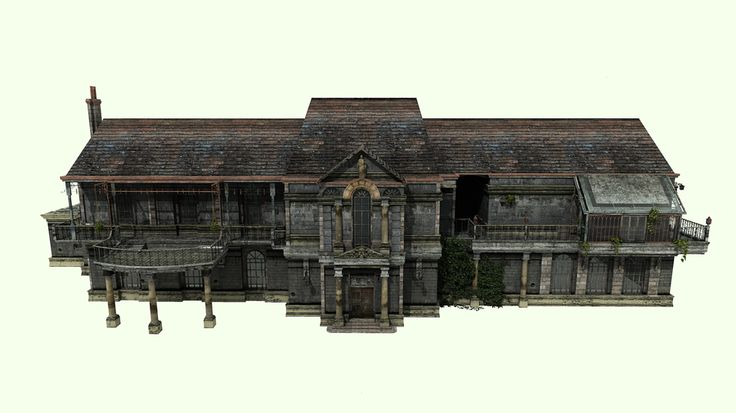
\includegraphics[width=\linewidth]{imgs/image.png}
        \caption{Imagem renderizada a partir de malha de polígonos. (\href{https://www.pinterest.com/pin/spencer-mansion--12807180169849484}){fonte}}
        \label{fig:mesh-polygon}
    \end{subfigure}
    \hspace{0.1\textwidth}
    \begin{subfigure}[b]{0.2\textwidth}
        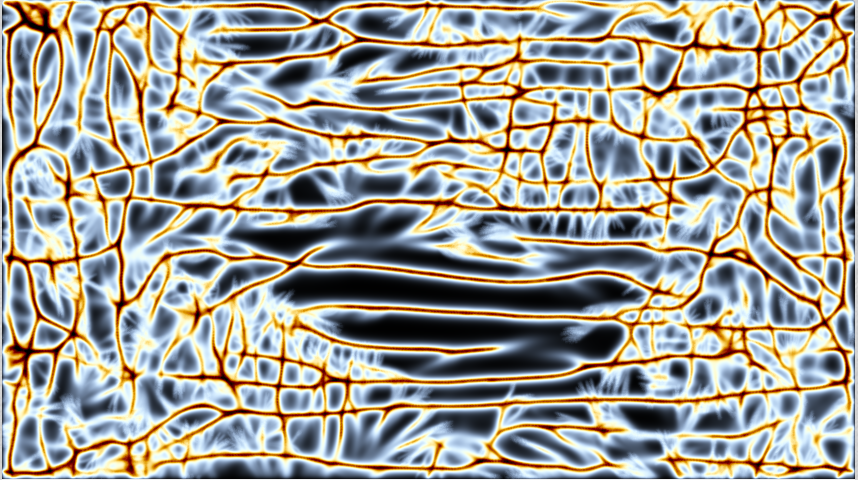
\includegraphics[width=\linewidth]{imgs/physarum.png}
        \caption{Imagem renderizada com algoritmo bio-inspirado. (\href{https://www.shadertoy.com/view/tlKGDh}{fonte}})
        \label{fig:physarum}
    \end{subfigure}
    \label{fig:sdl-images}
\end{figure}

\end{itemize}
\end{frame}

%------------------------------------------------

\subsection{Solução}
\begin{frame}{Solução}


\begin{itemize}
    \item \textbf{Gambiarra}: Para renderizar formas definidas e determinísticas mesmo sem input de objetos 3d, artistas técnicos utilizam de "campos de distância com sinal", que são uma forma de expressar um objeto tridimensional matemáticamente.
    
    \item \textbf{\textit{Signed Distance Fields}}: SDFs mapeiam à todo ponto do espaço um valor que representa a distância do determinado ponto à superfície mais próxima e caso o ponto esteja dentro da superfície parametrizada o valor da SDF é negativo.
\begin{figure}
    \centering
    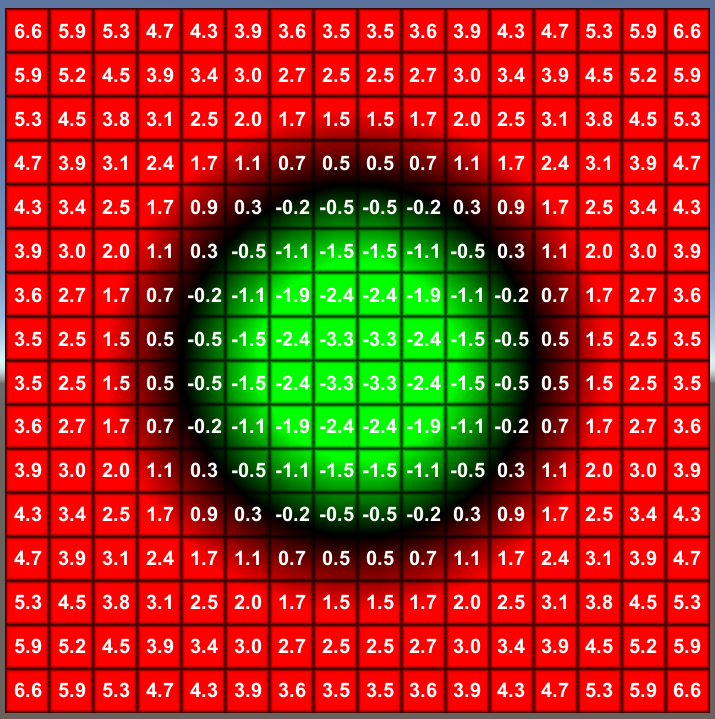
\includegraphics[width=0.25\linewidth]{imgs/SDF.png}
    \caption{SDF bidimensional de um círculo \href{https://shaderfun.com/2018/03/25/signed-distance-fields-part-2-solid-geometry/}{fonte}}
    \label{fig:enter-label}
\end{figure}
    
\end{itemize}



\end{frame}

%------------------------------------------------

\section{Renderizando SDFs}

\begin{frame}{Renderização SDFs}


\begin{itemize}
    \item \textbf{Raios:} Para renderizar cenas parametrizadas por sdfs, é necessário partir da posição da câmera e lançar raios que atravessam o plano da imagem a ser renderizada. Cada raio deve atravessar um pixel correspondente no plano da imagem e marchar em direção à cena.

    \begin{figure}
        \centering
        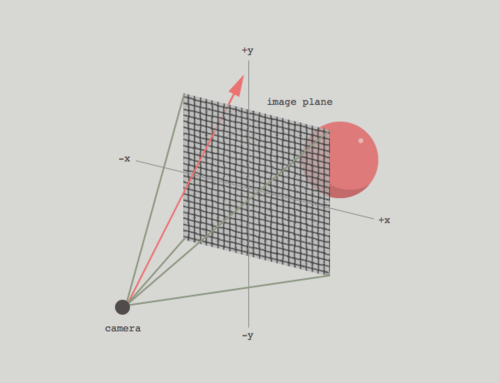
\includegraphics[width=0.5\linewidth]{imgs/image_plane.png}
        \caption{plano da imagem, \href{https://michaelwalczyk.com/blog-ray-marching.html}{fonte}}
        \label{fig:enter-label}
    \end{figure}

\end{itemize}


\end{frame}

\section{Renderizando SDFs}

\begin{frame}{Renderização SDFs}


\begin{itemize}
   
\item \textbf{Hit or Miss:} Os raios lançados são amostrados regularmente. Caso a distância em relação a alguma superfície calculada para uma dada amostragem de um raio seja menor que um \textit{"threshold"}, considera-se que o raio atingiu a superfície em questão. A amostragem desse raio é interrompida e a cor da superfície atingida é desenhada no pixel atravessado pelo raio.
\begin{figure}
    \centering
    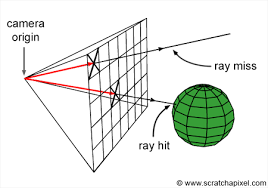
\includegraphics[width=0.4\linewidth]{imgs/hitOrMiss.png}
    \caption{Amostragem de um raio que atingiu uma superfície, o pixel atravessado pelo raio que atingiu a esfera deverá ser colorido de verde.
    \href{https://www.scratchapixel.com/lessons/3d-basic-rendering/ray-tracing-overview/ray-tracing-rendering-technique-overview.html}{fonte}
    }
    \label{fig:enter-label}
    \end{figure}
\end{itemize}
\end{frame}

\begin{frame}{Exemplos}
\begin{itemize}
\item As imagens finais renderizadas podem ser fantásticas e dependem apenas da capacidade do artista de escrever SDFs e funções de iluminação.

\begin{figure}
    \centering
    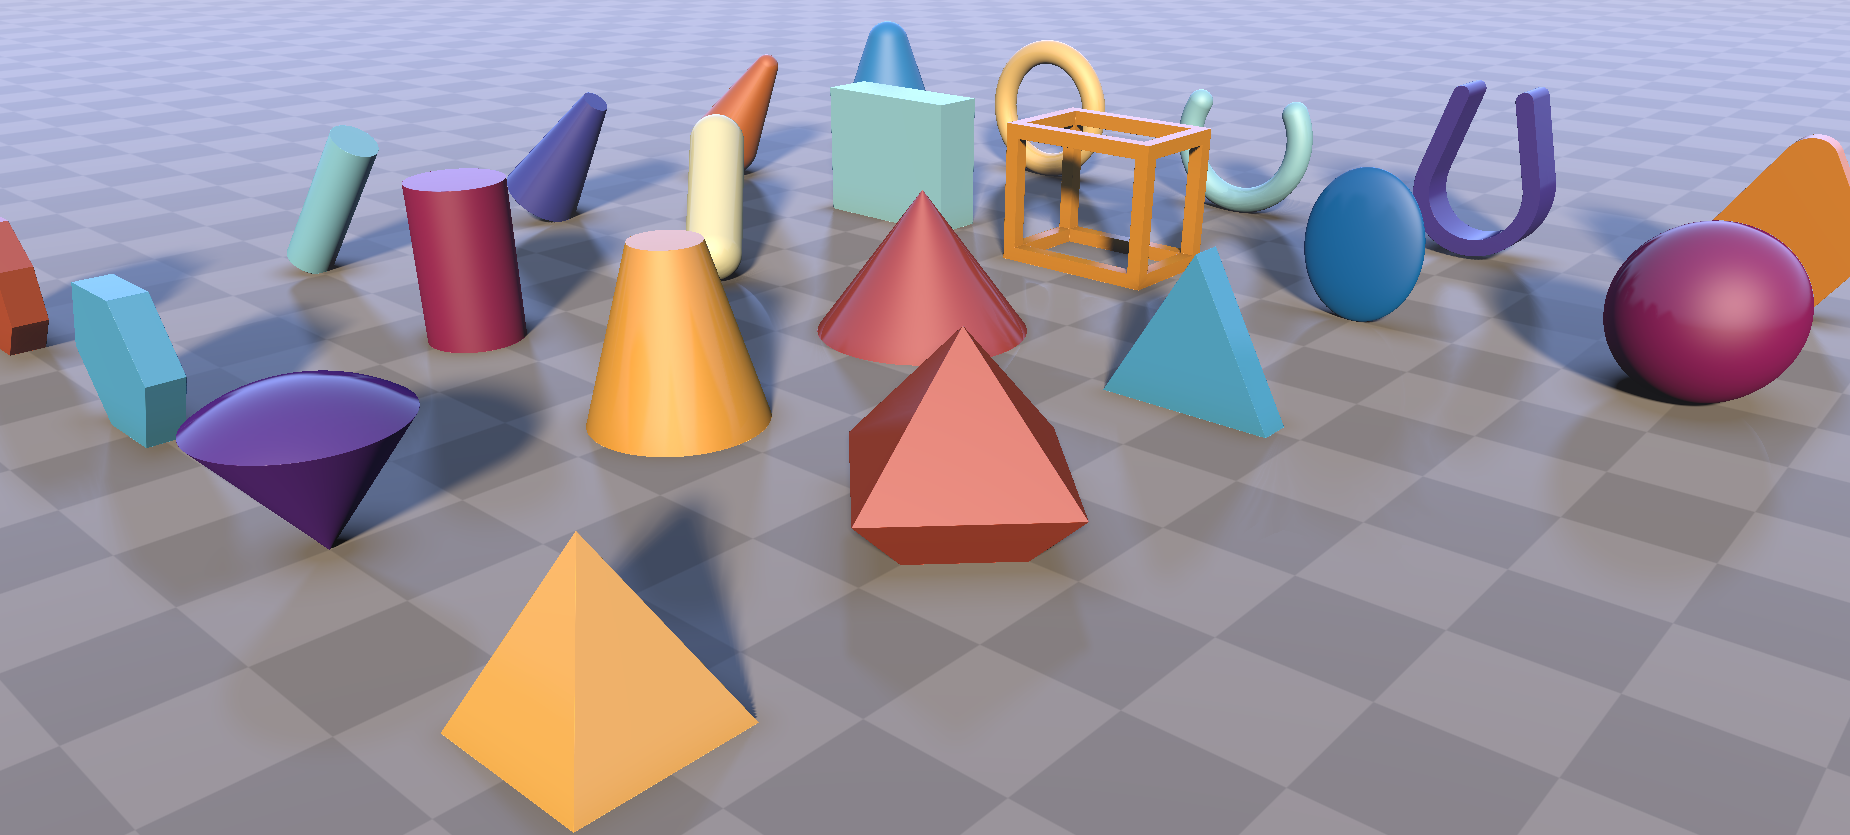
\includegraphics[width=0.5\linewidth]{imgs/iq.png}
    \caption{Artistas muito talentosos como Iñigo Quilez são capazes de criar cenas compostas por dezenas de SDFs diferentes. \href{https://www.shadertoy.com/view/Xds3zN}{fonte}}
    \label{fig:enter-label}
\end{figure}

\end{itemize}
\end{frame}

\begin{frame}{Linguagem}
\begin{itemize}
\item \textbf{SDL:} O objetivo então da linguagem é mais do que abstrair a construção do renderizador, abstrair também o processo de amostragem volumétrica da cena que chamamos de raymarching. Dessa forma, objetiva-se poder escrever apenas as funções de distância, funções de cor da cena e a linguagem vale-se do algoritmo de raymarching para renderizar a cena descrita pelo usuário na linguagem.
\end{itemize}
\end{frame}



%------------------------------------------------

\section{Exemplos}

\begin{frame}{Código 1 Exemplo}


\begin{figure}
    \centering
    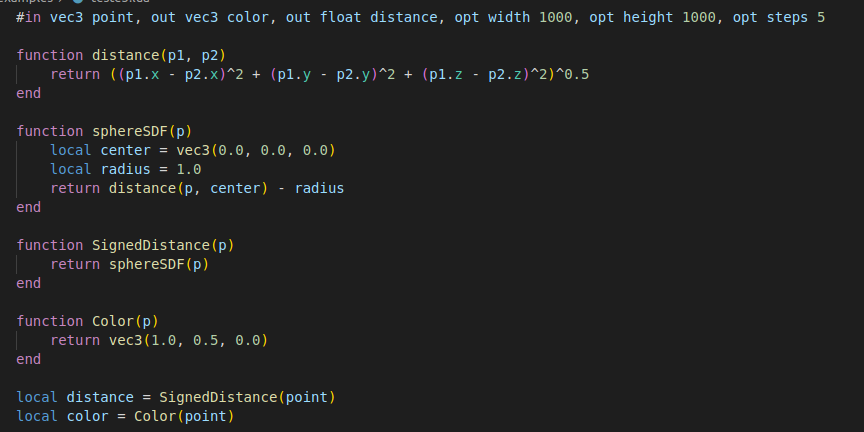
\includegraphics[width=0.7\linewidth]{imgs/exemplo_codigo.png}
    \caption{exemplo de código aceito pela linguagem.}
    \label{fig:enter-label}
\end{figure}
\end{frame}

%------------------------------------------------



\begin{frame}{Saída Exemplo 1}


\begin{figure}
    \centering
    
\includegraphics[width=0.5\linewidth]{imgs/ex1.png}
    \caption{Saída obtida para o primeiro exemplo}
    \label{fig:enter-label}
\end{figure}

\end{frame}

%------------------------------------------------
\begin{frame}{Código Exemplo 2}


\begin{figure}
        \centering
        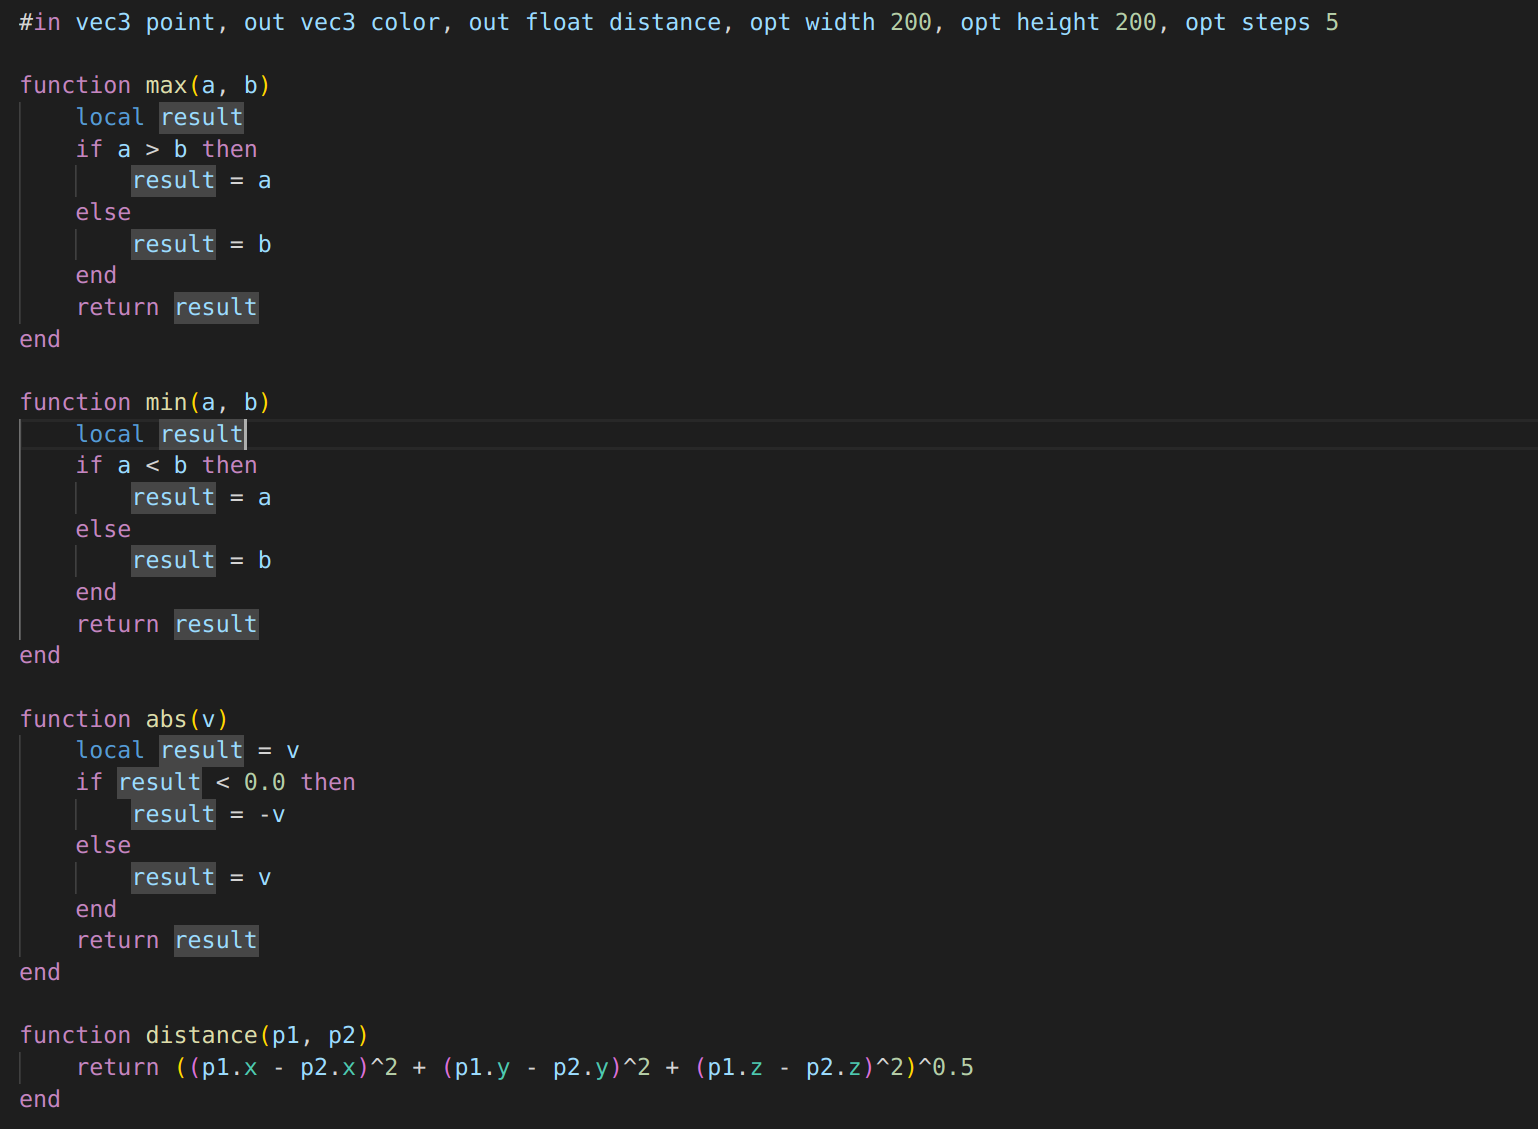
\includegraphics[width=0.7\linewidth]{imgs/cube1_code.png}
        \caption{Funções e diretivas de compilação para segundo exemplo.}
        \label{fig:enter-label}
    \end{figure}
\end{frame}

\begin{frame}{Código Exemplo 2}
\begin{figure}
    \centering
    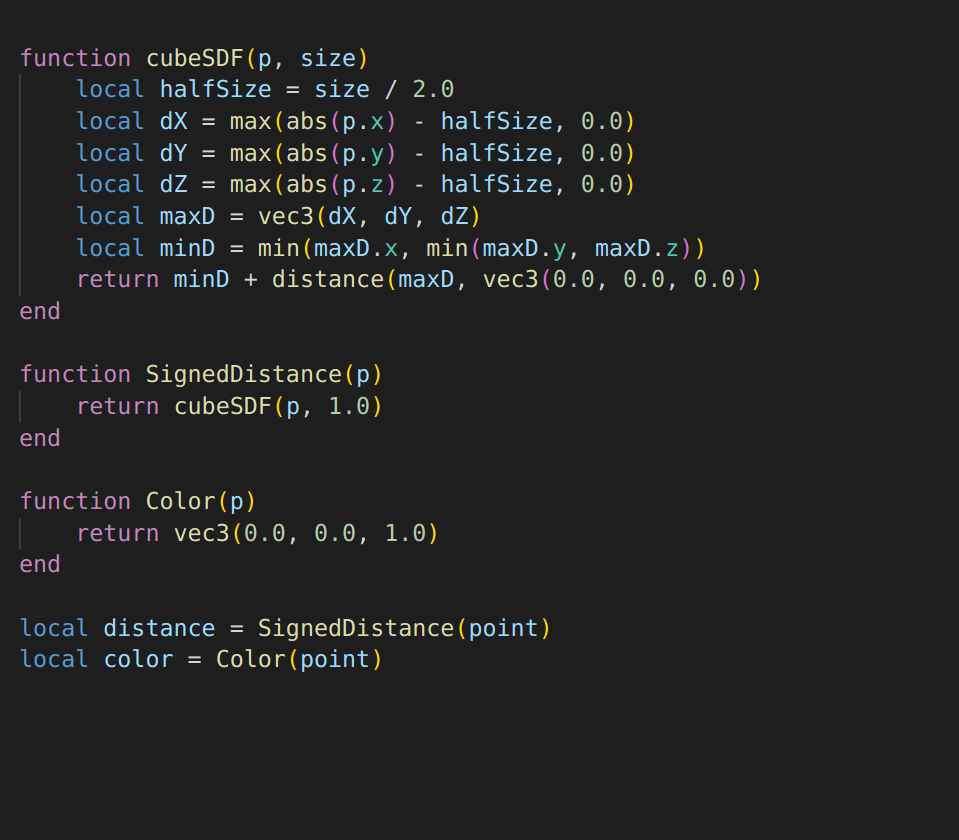
\includegraphics[width=0.7\linewidth]{imgs/cube2_code.png}
    \caption{Funções e diretivas de compilação para segundo exemplo.}
    \label{fig:enter-label}
\end{figure}
\end{frame}
    
    %------------------------------------------------
    
    
    
\begin{frame}{Saída Exemplo 2}
    
    
    \begin{figure}
        \centering
        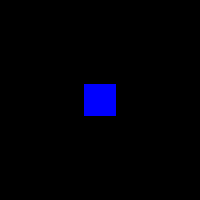
\includegraphics[width=0.5\linewidth]{imgs/cube.png}
        \caption{Saída obtida para o segundo exemplo}
        \label{fig:enter-label}
    \end{figure}
    
\end{frame}


%------------------------------------------------


%------------------------------------------------


\end{document} 